\section{Magic VLSI}

Jednym z bardziej popularnych oraz najbardziej dostępnych programów do projektowania układów scalonych
jest Magic VLSI\@.
Opracowany w 1983 roku przez Johna K. Ousterhouta i jego zespół na Uniwersytecie Kalifornijskim w Berkeley,
napisany w języku C, pierwotnie dla systemu Berkeley 4.2 będącego wariacją platformy Unix~\cite{MAGIC_article}.
Program ten posiada własną stronę internetową, na której można znaleźć dokumentację, kod źródłowy,
wskazówki dotyczące projektowania schematów, jak również pobrać program~\cite{MAGIC_site}.
Dzięki otwartemu kodowi źródłowemu oraz wysokiej funkcjonalności Magic zyskał dużą popularność
w środowiskach akademickich i naukowych, a także wśród hobbystów.
Jego główną jest brak konieczności posiadania płatnej licencji,
przy czym jednocześnie pozwala na pełne zaprojektowanie schematu układu scalonego.\\
\newpage
\indent Unikalną cechą programu Magic jest wprowadzenie techniki strukturyzacji danych
zszytych narożników \textit{corner-stitched},
która znacząco poprawia jego wydajność.
Mechanizm ten opiera się na reprezentacji układu scalonego jako zestaw warstw,
na które składa się zestaw prostokątnych komórek.
%(ang. \textit{cells}).
Każda komórka zawiera zszyte narożnikami powierzchnie (ang. \textit{corner-stitched planes}),
opisujące jej geometrię oraz podkomórki, a każda z nich składa się z wielu prostokątnych kafelków.
Taka struktura pozwala na szybkie i efektywne operacje na schemacie,
takie jak znajdywanie wszystkich kafelek w danym obszarze lub sąsiadów danej komórki,
a także przeszukiwanie połączonych regionów kafelków.
Dzięki zastosowanym mechanizmom możliwe jest także wykonywanie operacji na dużych obszarach
i szybką aktualizację danych.

\begin{figure}[h]
    \centering
    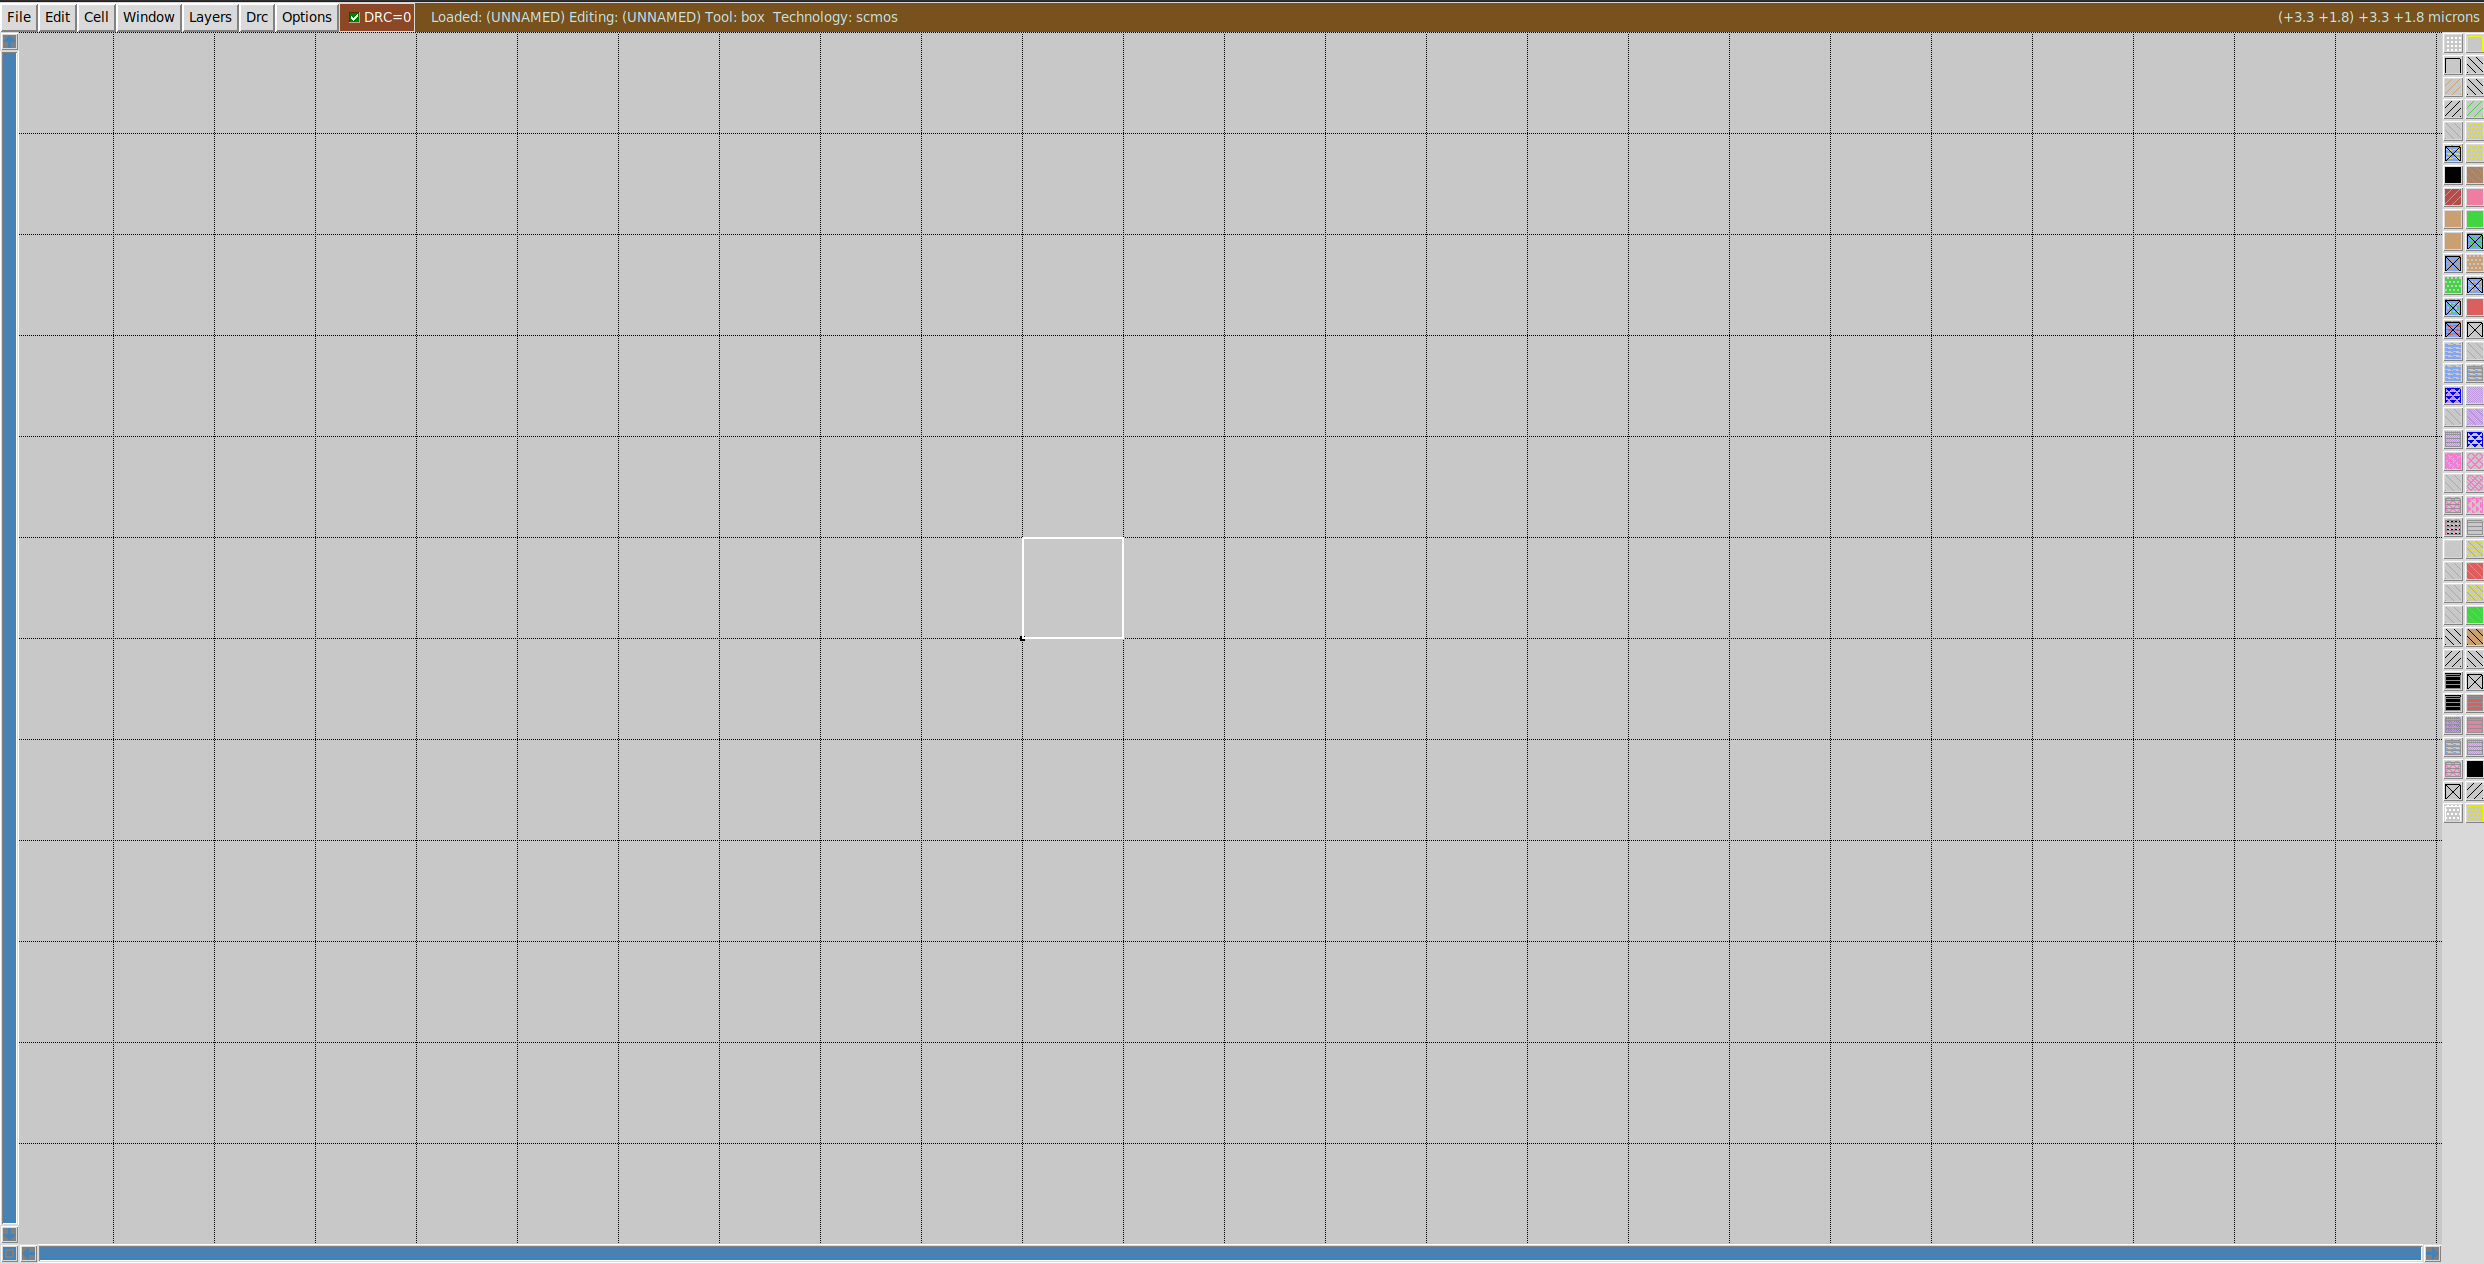
\includegraphics[width=\textwidth]{chapters/chapter2/img/magic_okno}
    \caption{Widok okna programu Magic VLSI.}
    \label{fig:magic_okno}
\end{figure}

\indent Magic VLSI posiada prosty interfejs graficzny,
który składa się z obszaru roboczego, paska narzędzi oraz paska wyboru materiałów.
Dodatkowo wraz z głównym oknem programu otwiera się okno konsoli pozwalające na wprowadzanie dodatkowych komend.
Rysowanie zaczyna się od zaznaczenia obszaru, lewy przycisk myszy służy do wyboru pozycji obszaru,
a prawy do jego rozszerzania.
Aby wypełnić obszar, należy wybrać odpowiedni materiał z paska wyboru
lub z już narysowanych komórek,
poprzez kliknięcie środkowym przyciskiem myszy.
%z tego powodu obecnie można go włączyć jedynie na systemach operacyjnych z rodziny Unix.

